\subsection{Introduction}
The term \textbf{brain (or neural) oscillations} refers to the rhythmic and/or repetitive
electrical activity generated spontaneously or in response to stimuli in the central nervous
system. The importance of brain oscillations in sensory-cognitive processes has become
increasingly evident. This chapter will focus on some questions:
\begin{itemize}
    \item What does a neural oscillation consist of and how does it originate?
    \item What are the (main) roles of brain oscillations?
    \item How do we observe a brain oscillation?
\end{itemize}

\subsection{EEG and MEG}
In the brain, what usually happens is that a current travels along the axons of the dendrites
generating an electrical field that is summed among many cells and finally reaches the
recording sensors, such as electrodes.\\
Electroencephalography (EEG) and Magnetoencephalography (MEG) are the main classical
techniques devoted to the electrical activity recording of the human brain in a non-invasive
way. They are based on systems that exploit the electrical field and the magnetic field,
respectively. Notice that generally they record two different aspects of the same event:
\begin{itemize}
    \item The EEG records the electrical field and, for this reason, the unit of measure
          is volts (typically
          microvolts, \(10^{-6}\,V\)).
    \item The MEG records the magnetic induced component in a static magnetic field where
          the head of the person is immersed. The unit of measurement is tesla (typically
          femtotesla, which corresponds to \(10^{-15}\,T\)).
\end{itemize}
One of the main differences between these two techniques is the acquisition system: EEG
uses sensors placed on the scalp and wires (one for each electrode) connected to an amplifier,
which is needed because the recorded electrical fields have a power that has to be magnified,
while MEG requires dedicated and specially built rooms and more intensive and expensive
maintenance. Another drawback of MEG is the fact that the coils used to acquire the signals
are fixed, hence, if the subject moves his head, there is a magnetic induction even though
no current is travelling, making data completely useless.\\
One of the main reasons to acquire and look at MEG instead of EEG is the fact that the
magnetic fields pass through the skull and scalp, whereas the electrical fields are volume
conducted through these tissues. This causes a decrease of the signal-to-noise ratio at
higher frequencies (performing a low-pass filtering). For this reason, MEG signals have a
better spatial resolution (better localization power), and this could be useful for instance
for clinical purposes, such as studying epilepsy.
\subsubsection{Origin of EEG Signals}
EEG is not so different from what has been said regarding local field potentials, but it has
one more problem caused by the fact that the sensors are not located into the brain, rather
outside it; thus, the signal has to travel all the way from the source up to the
electrodes. EEG is the synchronized synaptic activity in populations of cortical neurons
closer to the electrode, hence at the electrode end a spatial integration is performed (net
sum). The spatial integration is tightly related to the differences of \textbf{orientation}
between the neurons.\\
Electrodes detect the sum of positive and negative charges in their proximity. In the case
an electrode is equally distant from both the \textit{source} (region of positive charge) and the
\textit{sink} (region of negative charge) of a dipole, the electrode will measure a net
neutral charge; therefore, an electrode can only detect dipoles when it is closer to either
the positive or the negative end of the dipole. This means that mainly two types of dipoles
are measurable in EEG: \textbf{tangential dipoles}, which are perpendicular to the scalp
surface, and \textbf{radial dipoles}, which are parallel to it. Dipoles have a positive and
negative side, hence they can produce both a positive deflection and a negative deflection
in different regions of the scalp.
\begin{figure}[H]
    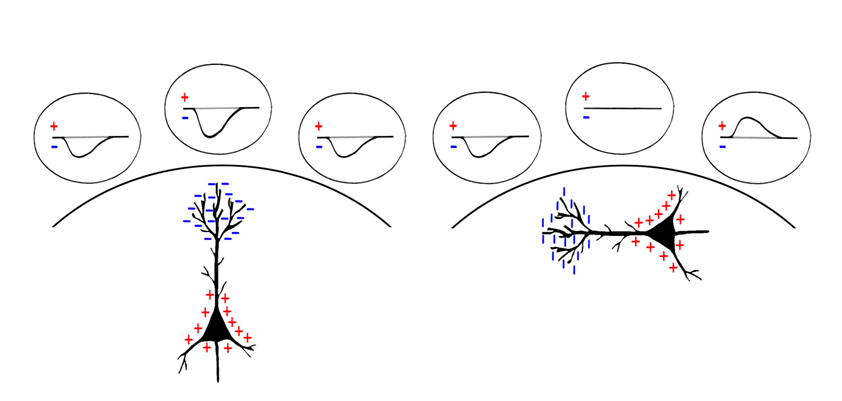
\includegraphics[scale=0.45]{10_1}
    \centering
\end{figure}
In general, a single-neuron dipole is too small to be measured at the scalp. However,
electrodes detect the sum of charges in their proximity, which in this case corresponds to
the sum of dipoles from multiple neurons, that can be considered as a single dipole whose
magnitude is proportional to the number of neurons whose dipoles are being summed together.
Anyway, since both positive and negative ends of dipoles in the brain are summed, in order to
produce a non-null signal, neurons must all be arranged in a \textit{parallel manner}, and
active in a \textit{synchronous way}. If this is not the case, the individual dipoles
positive and negative ends will cancel each other out.
\begin{figure}[H]
    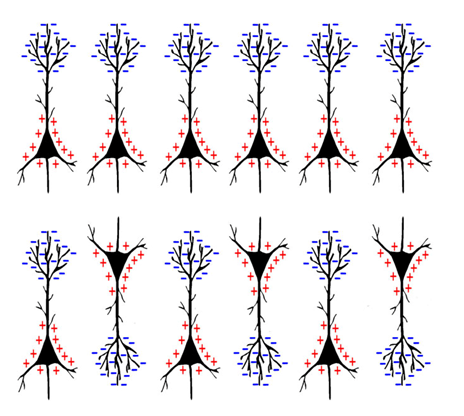
\includegraphics[scale=0.45]{10_2}
    \centering
\end{figure}
Finally, the electrical field moves in space to reach the sensors (due to the
\textbf{volume conduction} phenomenon). When the signal reaches the outer skull layers, if
there is no layer facilitating the passage of ions, it is not possible to record anything.
In order to deal with this issue, a conductive gel is commonly employed.
\begin{figure}[H]
    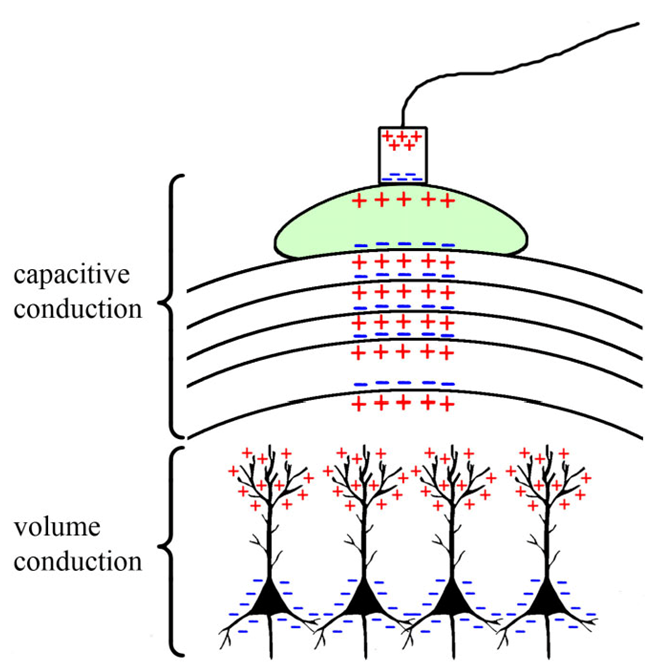
\includegraphics[scale=0.40]{10_3}
    \centering
\end{figure}
\subsubsection{EEG (Simplified) DAQ}
In the following picture a simplified model of the EEG acquisition system is reported:
\begin{itemize}
    \item The first element is the \textbf{sensor}, that has some resistance
          \(R_1\), representing the scalp.
    \item Then, there is a \textbf{cable}, used to connect the sensor to the amplifier.
          Its resistance is \(R_2\).
    \item The last part is the \textbf{amplification system}, with a resistance \(R_3\).
\end{itemize}
\begin{figure}[H]
    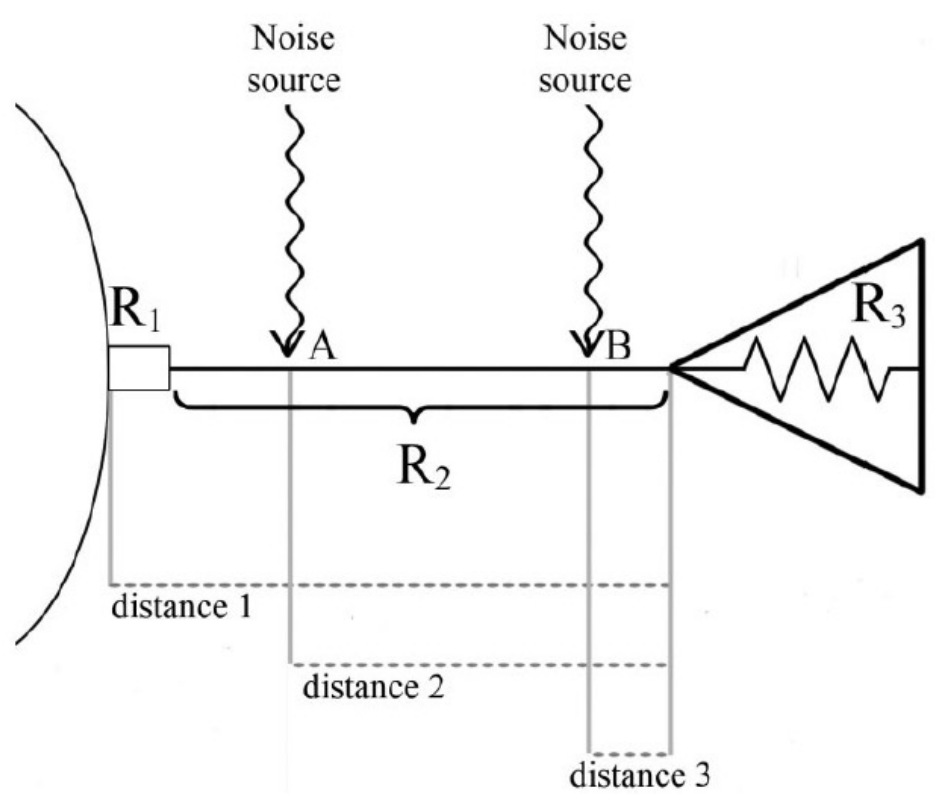
\includegraphics[scale=0.30]{10_4}
    \centering
\end{figure}
For the reasons mentioned earlier, \(R_1\) must be as low as possible to allow the ions to
reach the sensors. Also, the resistance of the cable \(R_2\) needs to be very small, in
order not to have any signal loss. On the other hand, \(R_3\) should be noticeably
large, compared to the other ones: it must be orders of magnitude larger than the sum of
the two. As a matter of fact, if the size of \(R_3\) were comparable to the ones of
\(R_1\) and \(R_2\), the largest fraction of the recorded activity would not be dependent on
the signal, but would be mainly noise, introduced by the sources \(A\) and \(B\).\\
Conversely, if a huge amplifier resistance is employed, what happens is that the potential
will be equally dependent from the noise and the signal itself and this allows to have a
better signal-to-noise ratio (SNR). Modern acquisition systems tend to improve these two
factors:
\begin{itemize}
    \item Increasing the amplifier input resistance (or impedance) \(R_3\).
    \item Reducing the distance between the amplifier and the sensors. A large slice of the
    modern systems exploit pre-amplification, performed directly nearby the sensors.
\end{itemize}
\subsubsection{EEG Principles and Good Practices}
A crucial question to ask when recording EEG data is: what does it need to be monitored to
obtain the best possible data?
\begin{enumerate}
    \item \textbf{Care in collection}: it is necessary to pay attention on the amount of gel
          introduced, depending on the quantity of channels on the top of the head and on the
          size of the head. If the electrodes are very close to each other, the conductive gel
          can create a so-called \textit{bridge}, coupling two sensors together.
    \item \textbf{Care in interpretation}: as said before, at the sensor level neurons can have
          many different orientations and this aspect must be taken into account. The dipoles
          measured by EEG consist of both positive and negative sides; a positive EEG
          deflection measured at a particular location will be balanced by a negative
          deflection elsewhere on the scalp. Thus, based only on the deflection of an EEG
          signal, an observer cannot infer whether the generator caused an excitatory or
          inhibitory current.
    \item \textbf{Care in localization}: the spatial resolution of the EEG is very poor,
          because of the volume conduction issue. Sources all over the brain may
          contribute to a signal measured on the scalp. The task of knowing only the final
          surface voltage pattern and working backwards to determine which sources within
          the brain produced that voltage pattern is the so-called \textit{inverse problem}.
\end{enumerate}
\subsubsection{EEG as a Critical-State System}
The activity acquired using EEG cannot be regarded as the product of a single part of the brain
acting as \textit{master} to explain the overall evolution of the system: the brain, such
as many other complex systems in nature, evolves in a so-called \textbf{critical dynamics}.\\
For this reason, the brain activity is not trivial, neither automatic nor repetitive: it evolves in
time and changes to different states. There is no interest in understanding how a single
neuron interacts with the others, but in evaluating how the system evolves and how
dynamically changes patterns of connectivity. To understand it, \textbf{brain oscillations}
can be studied.

\subsection{Constituents of Brain Oscillations}
Brain oscillations can be observed by looking at EEG signals (that have a very fast temporal
resolution, between \(200\,Hz\) and \(300\,Hz\)). Neuronal networks in the mammalian
forebrain demonstrate several oscillatory bands covering frequencies from approximately
\(0.05\,Hz\) to \(500\,Hz\).\\
Brain oscillations are observed in terms of mainly three elements:
\begin{itemize}
    \item \textbf{Frequency}: information on how fast the oscillation is travelling.
    \item \textbf{Phase}: information about the temporal occurency of a specific pattern.
    \item \textbf{Amplitude}: information on how large the oscillation is.
\end{itemize}
\begin{figure}[H]
    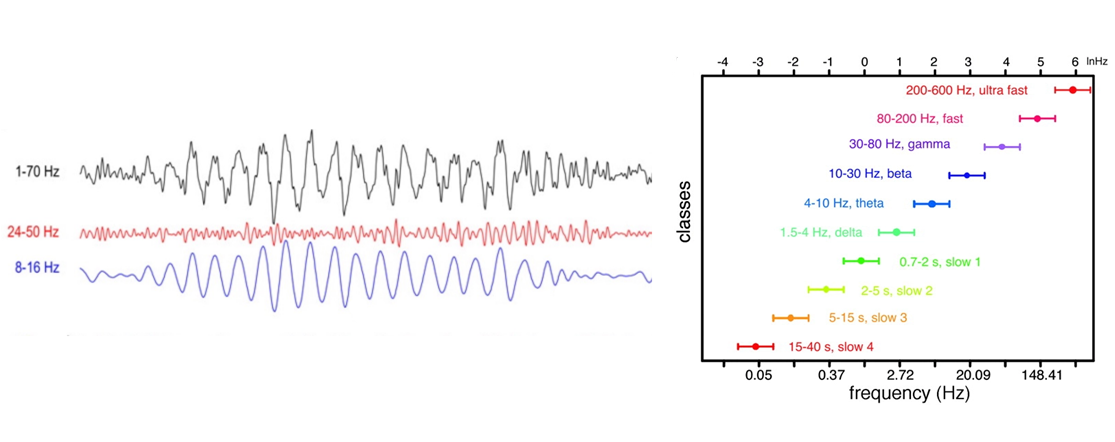
\includegraphics[scale=0.45]{10_5}
    \centering
\end{figure}
The figure above depicts the different Brain Bands or EEG Bands. A logarithmic scale is
used as the amplitude of EEG signals decays following a power-law behaviour; hence, the
representation is linear in a double-logarithmic scale.
\subsubsection{Oscillations Regulate Neuronal Processing}
Neurons communicate through spikes, but LFPs have the ability to control spikes: oscillations
are not just a secondary elements of the true activity, thus they are not epiphenomena.
\paragraph{Example}
Here two signals are recorded from different brain areas (Area \(A\) and Area \(B\)), having
access to both Local Field Potentials and spiking activity.
\begin{figure}[H]
    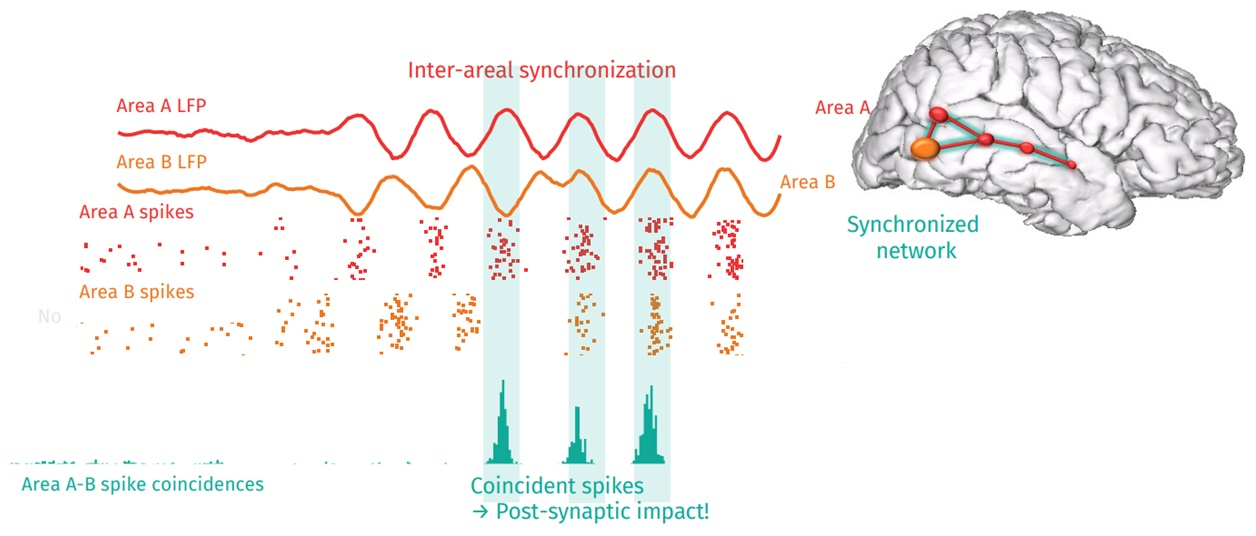
\includegraphics[scale=0.3]{10_6}
    \centering
\end{figure}
When the oscillations of the field potentials of the two regions are in opposite phase, the
region which generated the activity (the one that is trying to communicate) will be blocked
by the fact that the local field potential in the other region has a reduction in voltage
(that inhibits the voltage-dependent channels). If the oscillations are perfectly aligned,
what happens is exactly the opposite: if one brain region fires, the other responds,
producing an effective \textbf{communication}. This allows to conclude that
\textbf{temporal synchronization between field potentials is supportive for neural activity}.\\
By looking at the LFPs, it is possible to establish a link between physiology and cognition.
\subsubsection{Communication Through Coherence Theory}
Between 2005 and 2015, Fries P. formalized a theory called \textit{Communication through
coherence framework} and stating that if two populations have field activities that are
\textbf{coherent} in time - i.e., synchronized -, as soon as one stimulus reaches one population,
the same stimulus can also reach the other population. On the other hand, when the populations
are not aligned, given the fact that the oscillations control the excitation and the
excitatory cycle of the target cells, the signal will not propagate in the network.
\begin{figure}[H]
    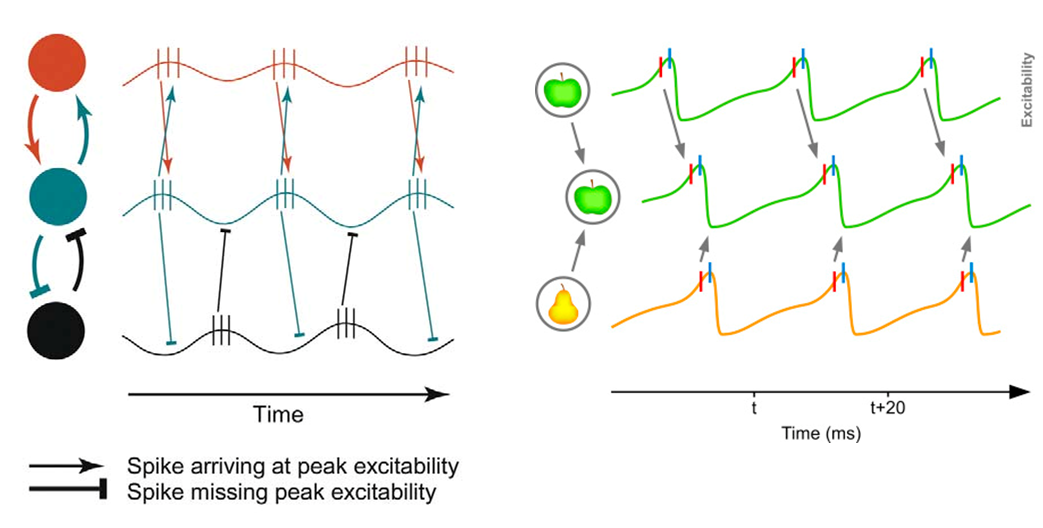
\includegraphics[scale=0.40]{10_7}
    \centering
\end{figure}
This framework can be directly applied to pairs of neurons, neuronal ensembles or even brain
regions, meaning that it is \textbf{scale-free}.\\
By looking at the second image, if there is a stimulation (first row), this is perceived by
all the populations whose excitation is perfectly in phase with the first one (second row).
The misalignment of the first two rows is consistent with the distance between the source and the
target. An example are Wernicke and Broca, that are two brain regions responsible for
understanding (Wernicke) and producing (Broca) language. They are connected by a
dense number of axons and the damage of one of the two regions could be a problem for
speaking or understanding language.\\
Hence, what has to be considered is not the perfect alignment in time of the two signals in
the different regions, but the fact that the misalignment between them - i.e., the time delay -
has to be coherent with the time that one signal requires to reach the other.\\
If this does not happen, for instance a third population (third row) receives a different
input and tries to communicate with the central region (second row), then the activity will
be blocked.
\subsubsection{Oscillations Regulate Context Switching}
On the basis of what has just been said, some structures that are physically linked can be
identified (for instance Wernicke and Broca areas), with respect to others whose
connection is more blurred (top level networks in the cognitive processing).\\
The brain needs to be able to switch among different configurations to process different
information simultaneously: this happens thanks to brain oscillations, that exist at all
frequency scales at the same time.
